W dobie dynamicznego wzrostu popularności aplikacji użytkowych na platformy mobilne (rys. \ref{figure:app_download}), oraz w momencie dynamicznego rozwoju technologii związanej z pojęciem Internet of Things, platformy mikroprocesorowe stają przed wyzwaniem zapewnienia funkcjonalności znanych z programów pisanych z myślą o jednostkach stacjonarnych oraz sprostaniem specyficznym wymaganiom dotyczącym rozmiaru, źródła zasilania i obsługi urządzeń nietypowych dla środowiska komputerowego .

Zarówno w przypadku oprogramowania obslugującego platformy mobilne \cite{bib:mobile-challenge}, jak i w przypadku koncepcji Internet of Things, nie zostały ustalone normy standaryzujące proces tworzenia oprogramowania, czy kontrukcji systemów opartych na połączeniu aplikacji webowych i mobilnych lub stacjonarnych. Za cel pracy przyjęto zaprojektowanie platformy mikroprocesorowej będącej zgodną z aktualnymi trendami rozwoju inżynierii internetowej. Wybory i założenia przyjęte podczas prac są tłumaczone, tak, by w oparciu o nich, móc odpowiedzieć na pytanie o granice adaptowalności, skalowalności i możliwości rozwoju systemów wbudowanych jako rozproszonego środowiska działania aplikacji użytkowych.

\begin{figure}[ht]
  \centering
  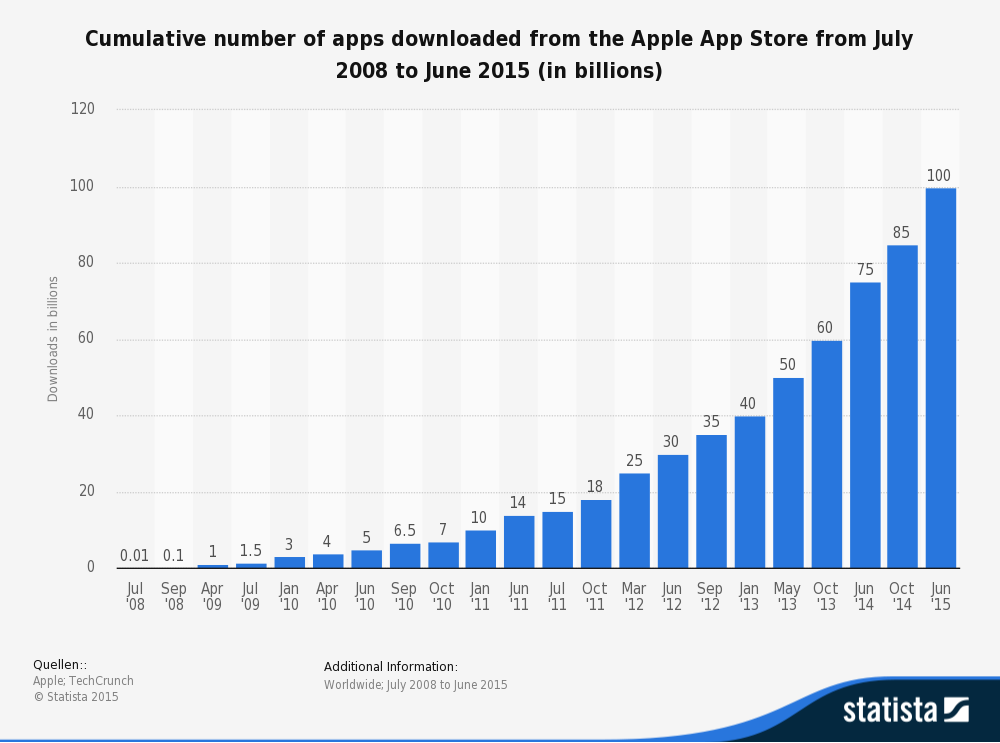
\includegraphics[width=\textwidth]{images/app_downloads.png}
  \caption{Wykres ilości pobrań aplikacji mobilnych dostosowanych do systemu operacyjnego popularnego producenta urządzeń mobilnych na przestrzeni ostatnich 7 lat.}
  \label{figure:app_download}
\end{figure}
\FloatBarrier



\subsection{Wymagania} % (fold)
Określenie wymagań stawianych projektowanemu systemowi zostało oparte o analizę potrzeb użytkownika na przykładzie aplikacji wspomagającej zarządzaniem czasem, oraz ogólno-przyjętymi wyznaczkami jakimi charakteruzją się aplikacje mobilne\cite{bib:mobile-paradigm}.


\label{sub:wymagania}
System przeznaczony jest dla pojedynczych użytkowników, do użytku własnego. Z tej perspektywy ważnymi, ale nie kluczowymi wyznacznikami urządzenia są:
\begin{enumerate}
	\item zapewnienie maksymalnej niezawodności
	\item wytrzymałość na zniszczenia i warunki ekstremalne
	\item możliwość wykonania kopii zapasowej
\end{enumerate}

Kluczowymi cechami platformy, ze względu na swoje przeznaczenie i środowisko pracy są:
\begin{enumerate}
	\item łatwe zarządzanie danymi
	\item trwałość i pewność zapisu
	\item wysoka dostępność do danych
	\item intuicyjność interfejsu aplikacji
	\item łatwa konfiguracja
	\item płynność działania aplikacji
	\item szybka synchronizacja
\end{enumerate}

Wymagania podstawowe stawiane aplikacji:
\begin{enumerate}
	\item możliwość anulowania operacji
	\item możliwość manipulacji danymi (dodawanie/edycja/usuwanie)
	\item interfejs w języku polskim
\end{enumerate}

Dostępność tłumaczy się jako możliwość podglądu zadań z poziomu aplikacji internetowej jak i aplikacji na platformach mikroprocesorowych zsynchronizowanych z aplikacją internetową.

% section wymagania (end)
\subsection{Ograniczenia} % (fold)
\label{sub:ograniczenia}
Ograniczeniem dla projektu są:
\begin{enumerate}
	\item wymiary
	\subitem platforma mikroprocesorowa powinna być możliwie płaska, oraz posiadać duży ekran dotykowy
	\item zasilanie
	\subitem systemy wbudowane wymagają specjalnego zasilania
	\item dostęp do internetu
	\subitem internet jest niezbędny do dwukierunkowej synchronizacji danych z serwerem
\end{enumerate}

Ograniczeniem dla projektu w przyszłości mogą być:
\begin{enumerate}
	\item przepisy regulujące kwestie związane z używaniem urządzeń elektrycznych w określonym środowisku (np. łazienka)
\end{enumerate}
